\section{Image Preprocessing}
\label{sec:image_processing}

\begin{wrapfigure}{R}[0pt]{0.45\textwidth}
	\vspace{-1.2cm}
	\centering
	
	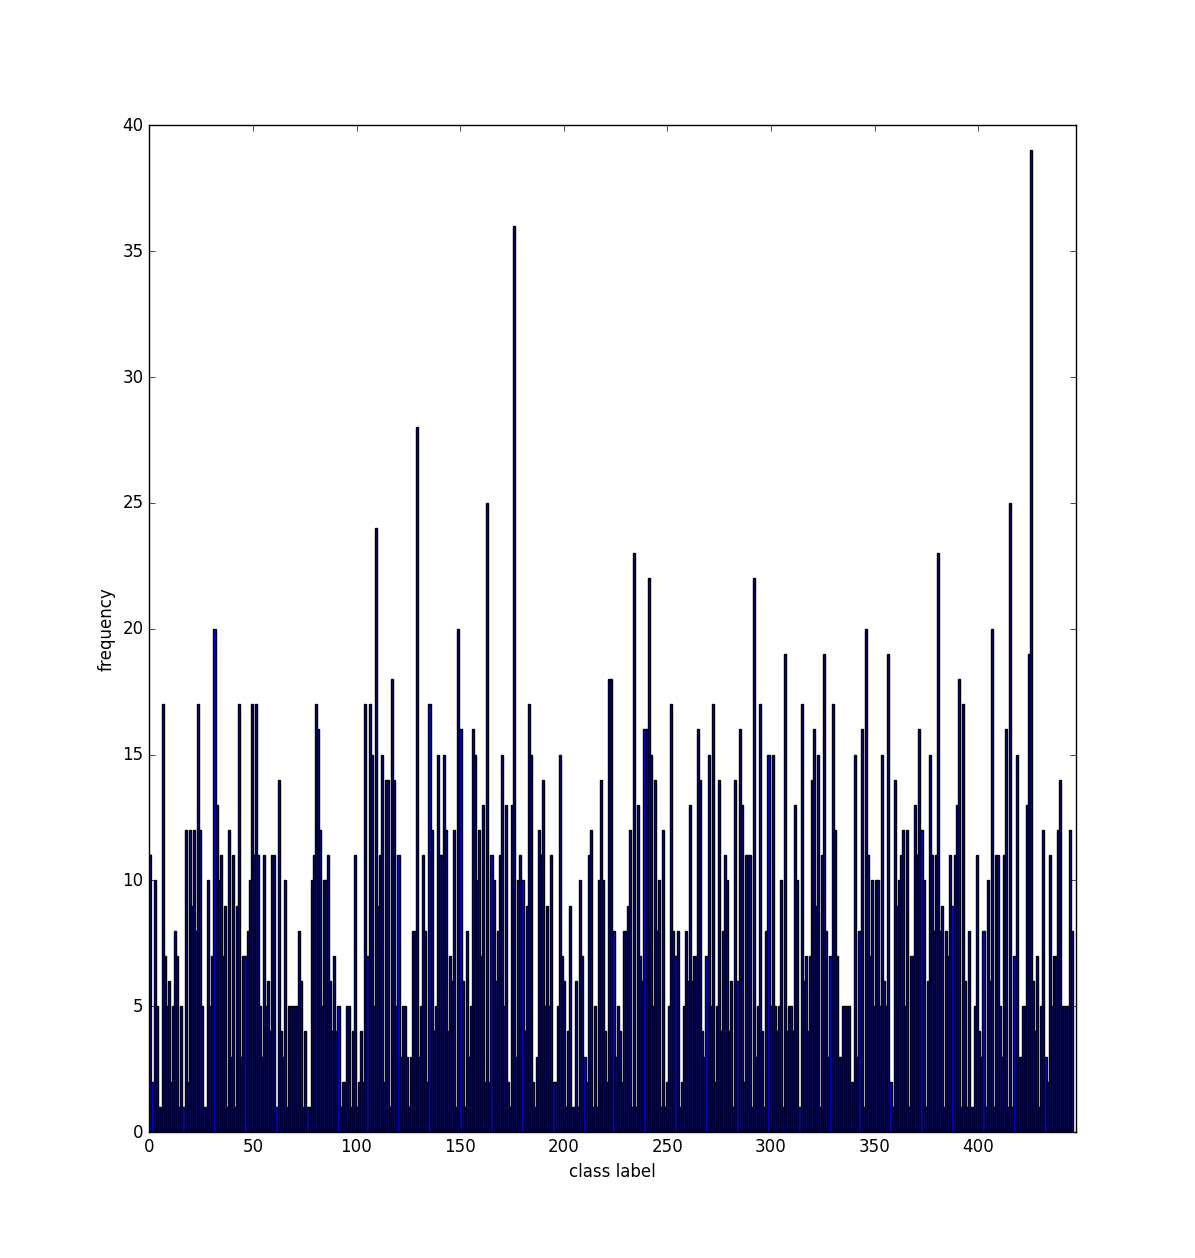
\includegraphics[width=0.45\textwidth]{sections/imgs/dataset/distribution.png}
	\caption{Dataset Distribution}
	\label{fig:dataset_distribution}
	
	\vspace{-1.0cm}
\end{wrapfigure}

The dataset given contains 11,468 images of 447 unique individual Right Whales. Figure~\ref{fig:right_whale_sample} is a sample aerial image of a whale contains large area of water and other noise around the whale body. The first challenge we faced was to segment and locate the Right Whale from the sea, we were particularly interested in the callosity patterns located on their heads, these unique features would enable us to identify different whales, other parts of the image are of negligible importance. Another challenge we faced was the fact that a large portion of Right Whales only have 1 or 2 images of an specific individual (see Figure~\ref{fig:dataset_distribution}), which means for those whales we have to use data augmentation techniques to increase the volume of the dataset.

Four different datasets were generated based from the original images. The general goal of this preprocessing stage is to eliminate variances that are not relevant to the classification task. The four prepocessing stages are as follows (\textbf{Note: We denoted the datasets with $D_{1}$, $D_{2}$. $D_{3}$. $D_{4}$, which will be used throughout this report}):

\begin{itemize}
	\vspace{-0.6cm}
	\setlength{\itemsep}{0pt}
	\setlength{\parskip}{0pt}
	\setlength{\parsep}{0pt}
	
	\item{$D_{1}$: Automated Head Cropping}
	\item{$D_{2}$: Manual Head Cropping}
	\item{$D_{3}$: Manual Head Cropping \& Rotation}
	\item{$D_{4}$: Applying Mask,Gabor Filter \& Clustering (K-Means \& DBScan)}	
\end{itemize}

\subsection{Automated Head Cropping ($D_{1}$)}
\label{subsec:auto_head_cropping}
\begin{wrapfigure}{R}[0pt]{0.4\textwidth}
	\vspace{-0.4cm}
	\centering
	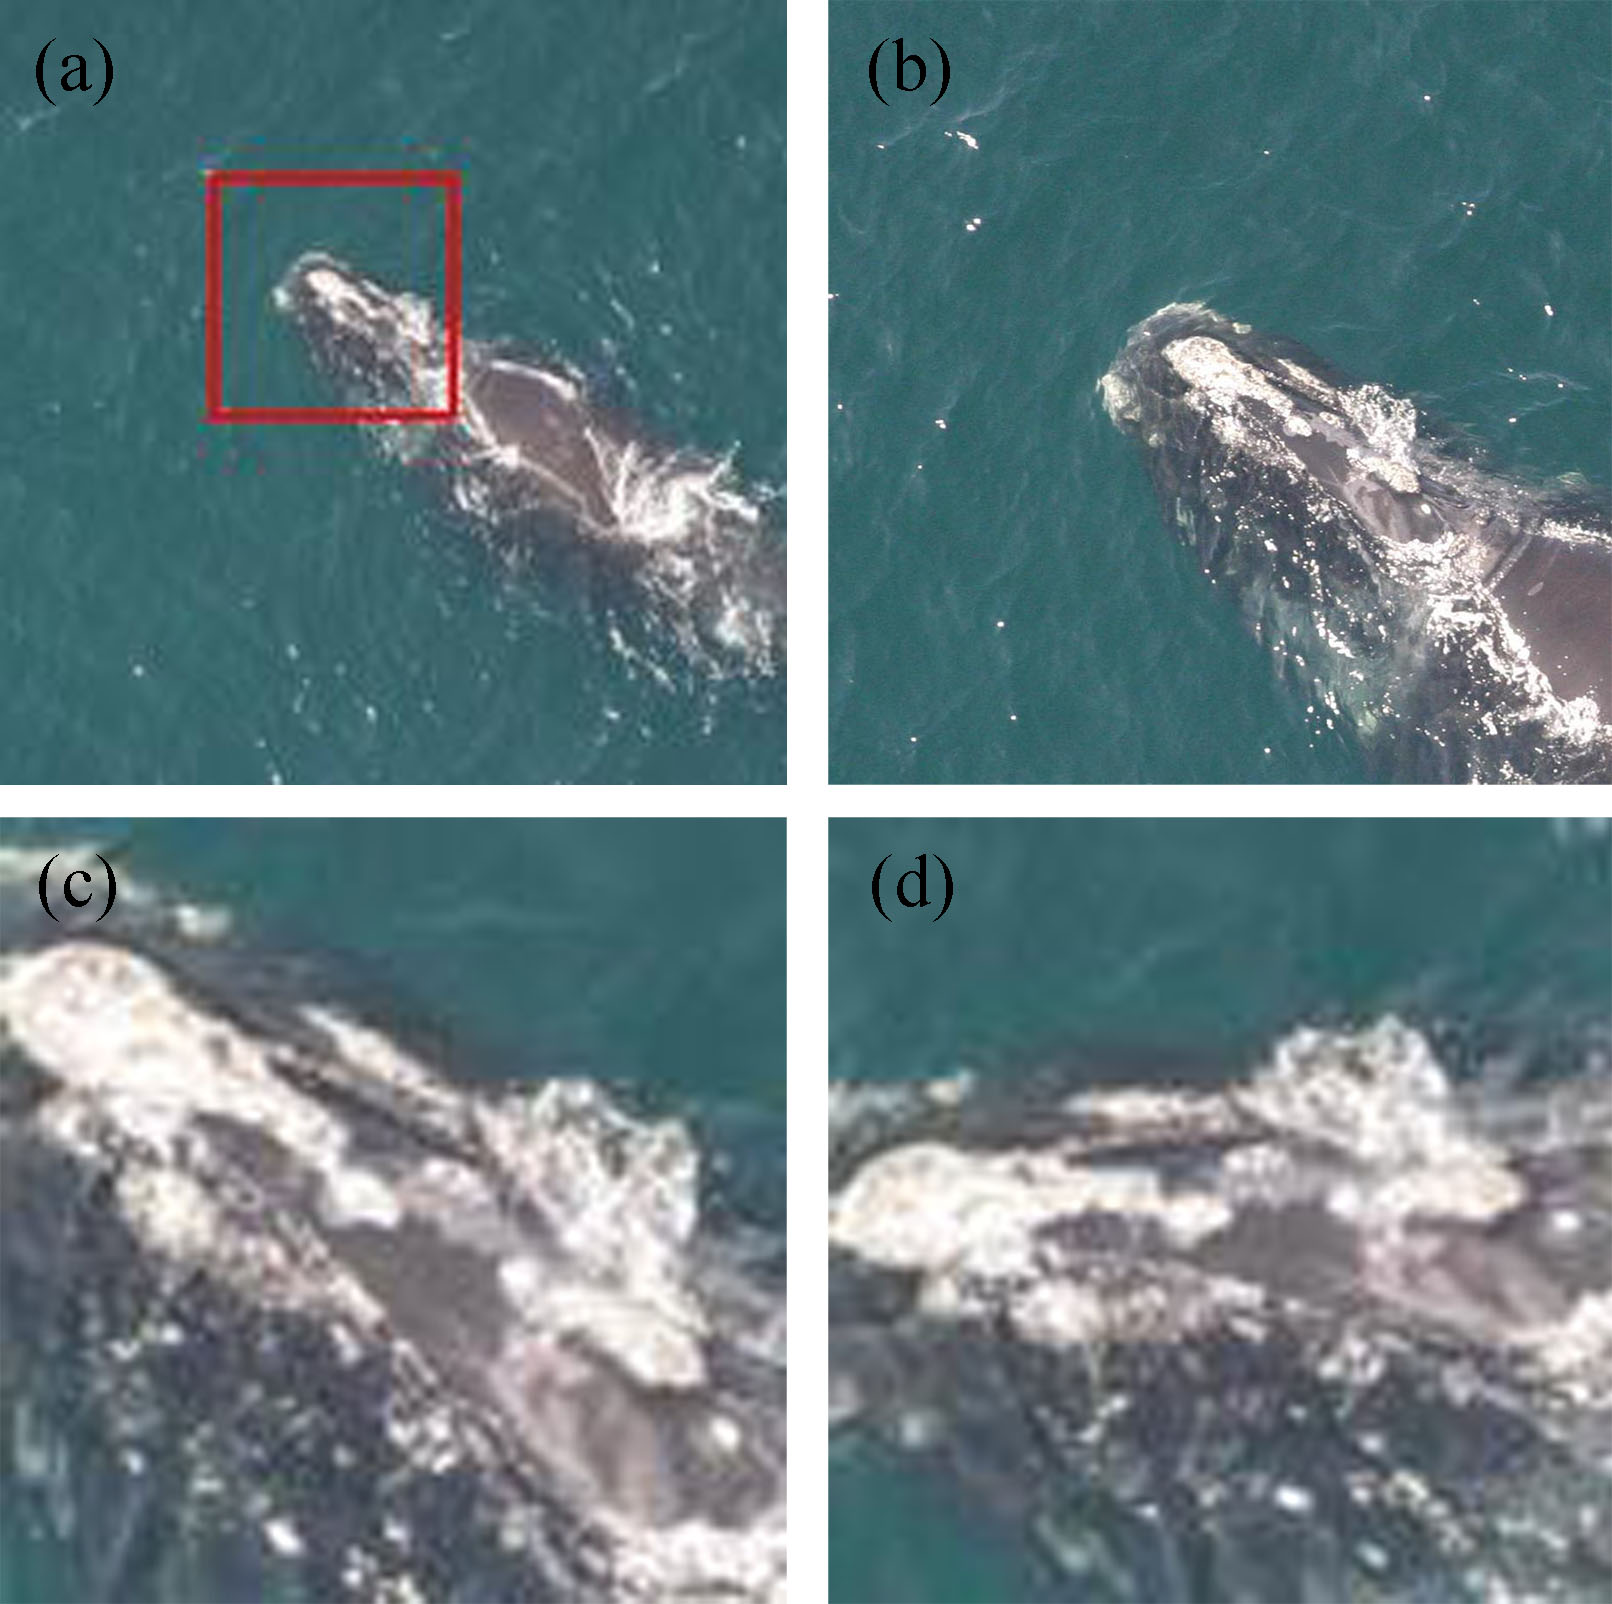
\includegraphics[width=0.35\textwidth]{sections/imgs/preprocessing/whale_image.jpg}
	\caption{Cropped whale images}
	\label{fig:preprocess_whaleimage}
\end{wrapfigure}
In our first attempt in segmenting and localizing the whale head we used a combination of techniques to automate this process. First we used a color-based thresholding method\cite{otsu1975threshold} on the blue channel to extract the sea background. Using thresholding method again this time on the gray channel, we can extract the whale body from the image. We then used Connected-component labeling\cite{haralock1991computer} to find the largest connected area which should contain the whale body. In-order to find the orientation of the whale the extracted whale body shape is fitted to an ellipse shape where regions of whale head and tail are assumed to be both ends of the long axis of the ellipse, this is performed using the centroidal profile approach\cite{davies2004machine}, where the contour of the head and tail sub-regions are transformed into polar coordinate system and comparing their regularities. This approach, however, is sensitive to variances in the image if in the image the whale is surfacing the water for air, creating lots of water waves around the whale body.

Using the automated process described above we found roughly 80\% (human inspection 40 out of 50) of the images contained correctly localized and segmented whale heads as shown in Figure~\ref{fig:preprocess_whaleimage}(a),(b). 20\% of the images however were not processed correctly and we had to process those manually. We can draw a conclusion that our preprocessing techniques is very sensitive to noise in the image and is only capable of localizing the whale head in an approximate fashion. See Supplementary Material~\ref{sup:auto_croping} for examples of the automated process.

As will be explained later, this dataset did not allow us to produce any meaningful classification results, as a result we generated the second dataset where the whale head is manually cropped for all images.

\subsection{Manual Head Cropping ($D_{2}$)}
\label{subsec:manual_head_cropping}
In our first attempt in creating $D_{1}$ we failed to create a robust method in segmenting and localizing the whale heads properly in an automated fashion, without spending further time into investigating automated techniques, we resorted to hand cropping the whale head images (see Figure\ref{fig:preprocess_whaleimage}(c)). The cropped images were then down-sampled to a resolution of $96 \times 96$ and subtracted the mean activity over this dataset from each pixel.


\subsection{Manual Cropping \& Rotation ($D_{3}$)}
\label{subsec:manual_cropping_and_rotation}
When we created $D_{2}$ it was not obvious to us that we had to align the whale head images in a uniform manner. This was made clear when we realized that Convolutional Neural Networks are not rotational invariant, thus as the next step, we rotated the manually cropped head images in a way that all the face patterns are aligned with the horizontal axis and centered in the image, as shown in Figure\ref{fig:preprocess_whaleimage}(d).


\newpage
\subsection{Mask \& Gabor ($D_{4}$)}
\begin{wrapfigure}{r}{0.35\textwidth}
	% \vspace{-0.8cm}
	\centering
	
\includegraphics[width=0.3\textwidth]{sections/imgs/preprocessing/kmeans.jpg}
	\caption{Image quantization using K-means}
	\label{fig:kmeans}
	%\vspace{-1.2cm}
\end{wrapfigure}
\label{subsec:mask_and_gabor}

From experiments we performed with $D_{1}$, $D_{2}$ and $D_{3}$ we found over-fitting to be a problem whilst applying different techniques (see Section~\ref{sec:methods_and_experimental_results}), also we hypothesized that dataset sparsity contributed to poor classification results, in many cases we had only 1 image per whale. We wanted to do a data Augmentation which would replicate the data and yet not introduce too much redundancy. One way was to randomly subsample the image. We thought that this could introduce a level of redundancy, since for this competition the featureset we had to focus on was very small (the pattern on the Whale Head). Also in many Images we had lots of water around the whale heads, randomly subsampling them would have caused the images to contain just water.

First we ran 2 Clustering Algorithms K-Means and DBScan to find the approximate location of the whale head pattern in the images. K-Means with $K = 4$ gave a better clustering result than the DBScan. The following figure shows the color quantization with K-Means.

\begin{wrapfigure}{r}{0.35\textwidth}
	\vspace{-0.6cm}
	\centering	
	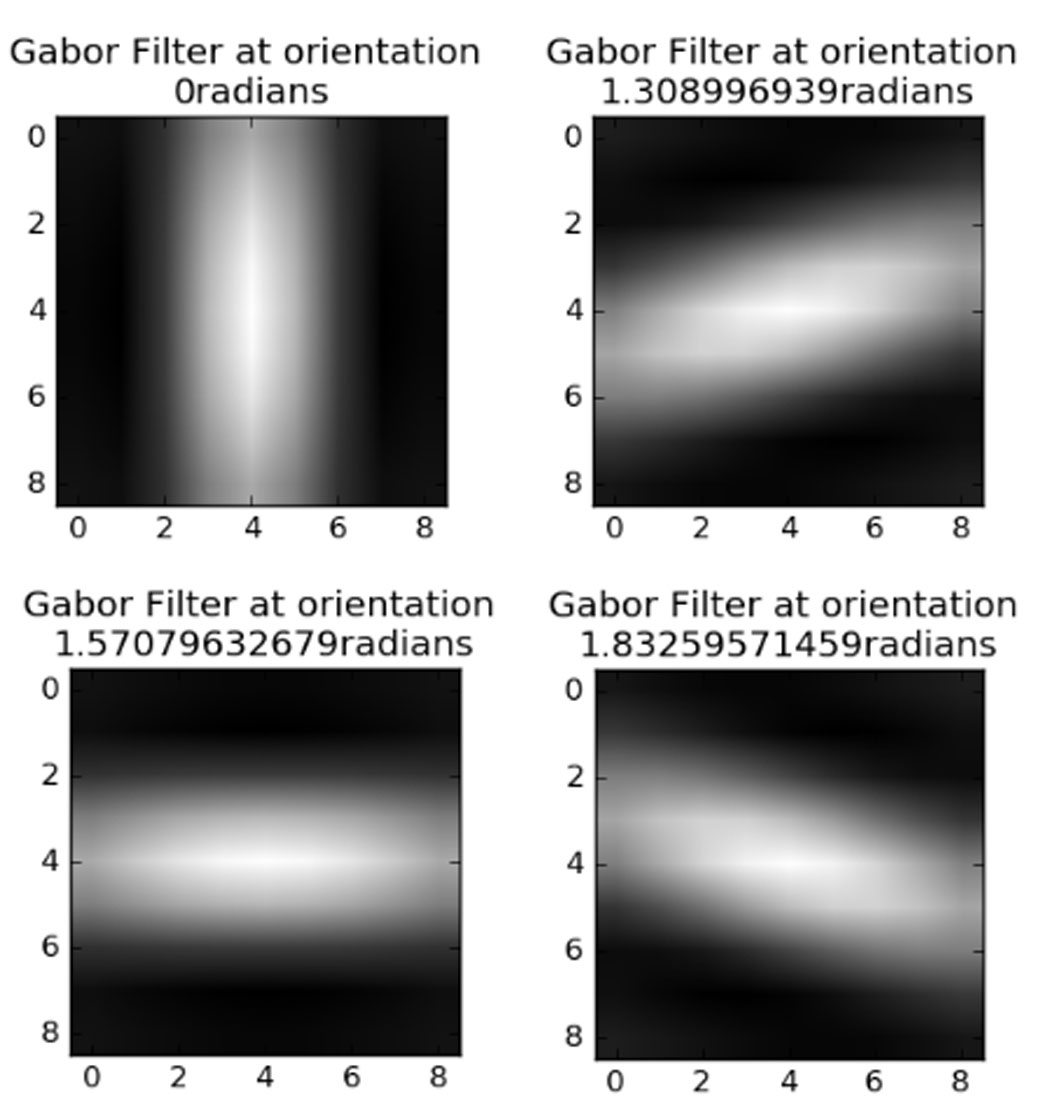
\includegraphics[width=0.35\textwidth]{sections/imgs/preprocessing/gabor_filter.jpg}
	\caption{Gabor Filters}
	\label{fig:gaborFilters}
	\vspace{-2.0cm}
\end{wrapfigure}

Gabor filters are bandpass filters which are used in image processing for feature extraction and  texture analysis. When a Gabor filter is applied to an image, it gives the highest response at edges and at points where texture changes. Frequency and orientation representations of Gabor filters are similar to those of the human visual system, and they have been found to be particularly appropriate for texture representation and discrimination. 

This approach was motivated by \cite{Gabor1} and \cite{Gabor2}

We used 4 Gabor Filters to augment the data, and applied to the image as well as the horizontally flipped image. So, in all we had 10 images per original whale image. We experimented with different configartions of Gabor Filters, the following parameters worked best $\nu = 1/9$ , $\sigma = 2.0$ , $\text{kernel size} = 9 \times 9$ ,and $\theta = 0, \frac{5\pi}{12}, \frac{\pi}{2}, \frac{7\pi}{12}$.
%\begin{figure}[H]
%	\centering
%	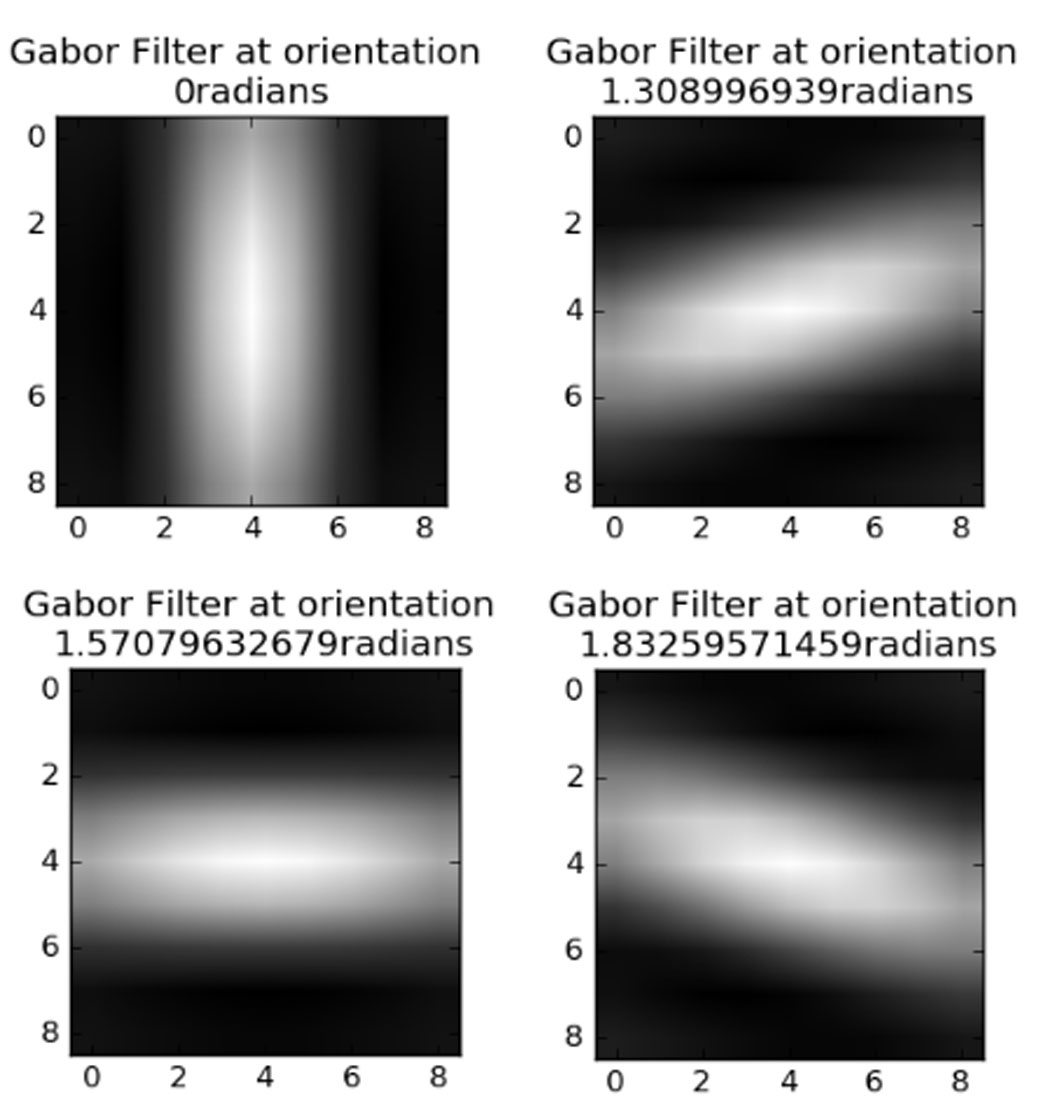
\includegraphics[scale=0.35]{sections/imgs/preprocessing/gabor_filter.jpg}
%	\caption{Gabor Filters}
%	\label{fig:gaborFilters}
%\end{figure}

After preparing the datasets, We applied four deep learning methods to Recognize whales.In the next section, the deep learning methods and the obtained results are described in detail.
